\chapter{实验环境搭建}

\section{仿真环境配置}

\subsection{Carla 仿真平台}

Carla 是一个开源的自动驾驶仿真平台,提供高度逼真的交通场景和车辆动力学模型。在本研究中,我们选择 Carla 的 Town10 仿真场景作为实验环境,该场景包含多个交叉路口、不同类型的车道以及丰富的交通元素,能够模拟真实交通场景中的各种复杂情况,为多目标跟踪算法的测试提供了良好的基础\cite{卢嘉伟 2025 复杂环境下自动驾驶汽车视觉目标检测模型性能评估}。

版本选择:安装 Carla 0.9.15 版本,该版本在功能和稳定性方面能够满足我们的实验需求。
场景加载:通过 Carla 的客户端程序加载 Town10 场景,确保场景中的道路、建筑物、交通标志等元素正确加载并显示。

传感器配置:在 Carla 中为车辆配置多种传感器,包括 RGB 相机、深度相机和激光雷达等。RGB 相机用于获取交通场景的视觉图像,深度相机和激光雷达则提供目标物体的距离信息,这些传感器数据将作为多目标跟踪算法的输入。根据实验需求,合理设置传感器的参数,如分辨率、帧率、视场角等,以获取高质量的仿真数据\cite{田卓灵 2011 自动驾驶}。

\subsection{Pycharm环境配置}
根据课题要求,本项目进一步搭建了与 Town10 仿真场景相关的交通数字孪生环境,用于获取目标的真实跟踪轨迹(Ground Truth)以及优化检测跟踪模型。

环境搭建:首先,根据项目与课题的要求,创建 Python 3.8 的虚拟环境,并安装如表~\ref{tab:full-dependencies} 所示的关键依赖包

\begin{table}[htbp]
	\centering
	\caption{Python 虚拟环境完整依赖清单}
	\label{tab:full-dependencies}
	\begin{tabular}{lll}
		\hline
		\textbf{类别} & \textbf{包名称} & \textbf{版本} \\ 
		\hline
		\multirow{8}{*}{核心依赖}
		& numpy & 1.24.4 \\
		& scipy & 1.10.1 \\
		& protobuf & $\geq$3.6 \\
		& future & $\geq$0.16.0 \\
		& psutil & 6.1.0 \\
		& opencv-python & 4.10.0.84 \\
		& pillow & 10.4.0 \\
		& open3d & 0.18.0 \\
		
		\hline
		\multirow{6}{*}{仿真交互}
		& carla & 0.9.15 \\
		& pygame & $\geq$1.9.4 \\
		& pywin32 & 308 \\
		& configargparse & 1.7 \\
		& retrying & 1.3.4 \\
		& tenacity & 9.0.0 \\
		
		\hline
		\multirow{7}{*}{数据处理}
		& pandas & 2.0.3 \\
		& python-dateutil & 2.9.0.post0 \\
		& pyparsing & 3.1.4 \\
		& contourpy & 1.1.1 \\
		& cycler & 0.12.1 \\
		& fonttools & 4.55.1 \\
		& packaging & 24.2 \\
		
		\hline
		\multirow{6}{*}{可视化}
		& matplotlib & 3.7.5 \\
		& plotly & 5.24.1 \\
		& dash & 2.18.2 \\
		& dash-core-components & 2.0.0 \\
		& dash-html-components & 2.0.0 \\
		& dash-table & 5.0.0 \\
		
		\hline
		\multirow{8}{*}{开发工具}
		& ipython & 8.12.3 \\
		& jedi & 0.19.2 \\
		& traitlets & 5.14.3 \\
		& prompt-toolkit & 3.0.48 \\
		& pygments & 2.18.0 \\
		& wcwidth & 0.2.13 \\
		& platformdirs & 4.3.6 \\
		& executing & 2.1.0 \\
		
		\hline
		\multirow{6}{*}{Web框架}
		& flask & 3.0.3 \\
		& werkzeug & 3.0.6 \\
		& jinja2 & 3.1.5 \\
		& itsdangerous & 2.2.0 \\
		& click & 8.1.8 \\
		& blinker & 1.8.2 \\
		
		
		
		\hline
	\end{tabular}
\end{table}

航点控制与轨迹平滑:利用项目中的航点控制模块,获取车辆在 Town10 场景中的运行航点。通过轨迹平滑算法生成连续轨迹,主要依赖 scipy 的信号处理模块和 numpy 的数值计算功能,相关算法实现基于表~\ref{tab:full-dependencies} 中的科学计算库。

PID 控制器:采用 PID 控制算法对车辆进行控制,其核心实现依赖 numpy 进行矩阵运算,同时利用 matplotlib 进行控制过程可视化。表~\ref{tab:full-dependencies} 中列出的实时数据可视化工具 dash 用于构建控制参数调试界面\cite{方虹苏 2025 基于深度强化学习的智能汽车控制模型研究}。

\subsection{Matlab环境配置}

版本:Matlab2024b


\begin{figure}[htbp] % 可以是h(here),t(top),b(bottom),p(page of floats)
	\centering
	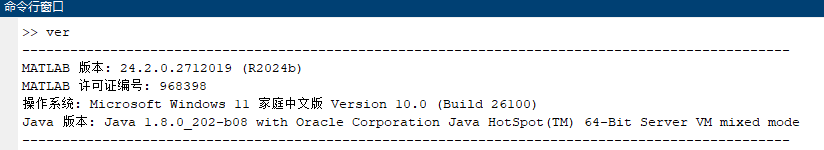
\includegraphics[width=1\textwidth]{p7} % 假设图片文件名为car.pdf或car.png等,位于当前工作目录
	\caption{matlab环境} % 图片标题
	\label{fig:p7} % 用于引用的标签
\end{figure}


MATLAB 是一个功能强大的算法开发平台,其提供的图像处理工具箱(Image Processing Toolbox)和计算机视觉工具箱(Computer Vision Toolbox)为多目标跟踪算法的开发提供了丰富的函数和工具。可以利用这些工具箱快速实现和测试各种多目标跟踪算法,如基于卡尔曼滤波(Kalman Filter)、联合概率数据关联滤波(JPDAF)等的经典算法,以及结合深度学习的目标检测和跟踪算法。通过在 MATLAB 中实现这些算法,可以方便地对算法的性能进行评估,调整算法参数,并与现有的 Baseline 算法进行对比分析。
在实验中,由于收集到的数据量较大且复杂,MATLAB 提供了丰富的数据处理工具箱,如信号处理工具箱(Signal Processing Toolbox)和统计与机器学习工具箱(Statistics and Machine Learning Toolbox),能够高效地对交通场景中的传感器数据进行预处理、特征提取和统计分析。例如,可以使用这些工具箱对从 Carla 仿真平台获取的车辆轨迹数据进行滤波处理,去除噪声,提取关键特征点,并对多目标的运动模式进行建模和分析\cite{穆凡 2025 神经先验增强的抗干扰鲁棒自动驾驶导航}。


\begin{figure}[htbp] % 可以是h(here),t(top),b(bottom),p(page of floats)
	\centering
	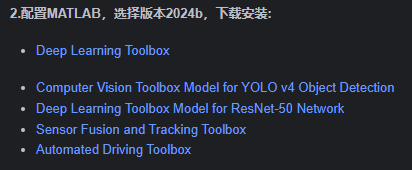
\includegraphics[width=1\textwidth]{p8} % 假设图片文件名为car.pdf或car.png等,位于当前工作目录
	\caption{matlab配置} % 图片标题
	\label{fig:p8} % 用于引用的标签
\end{figure}






\section{实验设备与软件工具}

\subsection{硬件设备}

设备名称:DESKTOP-H2JCRHP

处理器:AMD Ryzen 7 5800H with Radeon Graphics            3.20 GHz

机带:RAM	16.0 GB (15.4 GB 可用)

设备 ID:9FF8ABE5-216E-4C15-B738-D4364271428F

产品 ID:00326-40000-00000-AAOEM

系统类型:64 位操作系统, 基于 x64 的处理器

GPU:NVIDlA GeForce RTX 3060 Laptop GPU 与 Radeon(TM) Graphics

内存:1.32TB

该硬件配置能够满足 Carla 仿真平台的运行需求,同时保证多目标跟踪算法的高效训练和测试。配备大容量的固态硬盘(SSD),用于存储 Carla 仿真场景数据、传感器采集的数据以及实验过程中产生的大量模型文件和结果数据,确保数据的快速读写和存储安全。



\subsection{软件工具}

操作系统:Windows 11

编程语言与开发工具:主要使用 Python 语言进行算法开发和实验脚本编写,借助 PyCharm,提供代码编辑、调试、版本控制等功能,提高开发效率。同时,安装 carla、NumPy、SciPy、OpenCV 等常用 Python 库,用于数据处理、图像处理和数学计算等操作。

深度学习框架:采用 PyTorch 深度学习框架,其具有灵活的模型构建方式和强大的自动微分功能,便于我们实现和优化多目标跟踪模型。通过安装 PyTorch 及其相关依赖包,如 torchvision 等,为模型的训练和测试提供支持。

数据库管理系统:使用 MySQL 数据库管理系统,用于搭建路口车辆航点到 Carla 坐标映射的数据库。通过创建相应的数据表,存储路口、车道、方向等信息以及对应的 Carla 场景中道路终点坐标位置(x, y, z 和 yaw),为路口导航和目标跟踪提供数据支持。

可视化工具:MATLAB 具有强大的可视化功能,能够以二维或三维图形的形式直观地展示多目标跟踪的结果。例如,在实验中,可以使用 MATLAB 的绘图函数绘制车辆在 Town10 仿真场景中的运动轨迹,将不同目标的轨迹用不同的颜色或样式区分,从而清晰地观察和分析目标的运动情况和算法的跟踪效果。此外,还可以利用 MATLAB 的图形用户界面(GUI)设计工具,如 App Designer,开发定制化的可视化界面,方便用户与实验数据和算法结果进行交互。借助 Matplotlib、Seaborn 等 Python 可视化库,以及 Carla 自带的可视化工具,对多目标跟踪算法的结果进行可视化展示。通过绘制目标轨迹图、性能指标曲线等,直观地呈现算法的性能和效果,便于分析和比较不同模型之间的差异


